\PassOptionsToClass{10pt,conference}{IEEEtran}
\documentclass[class=IEEEtran,border=4pt]{standalone}
\usepackage{amsmath,amssymb}
\usepackage{xcolor}
\usepackage{tikz}
\usetikzlibrary{patterns,decorations.pathmorphing,calc,positioning}

% LfD colour palette (matches config.R)
\definecolor{lfdTeal}{HTML}{009371}
\definecolor{lfdRed}{HTML}{ED665A}
\definecolor{lfdOrange}{HTML}{E69F00}
\definecolor{lfdBlue}{HTML}{1F78B4}

\begin{document}
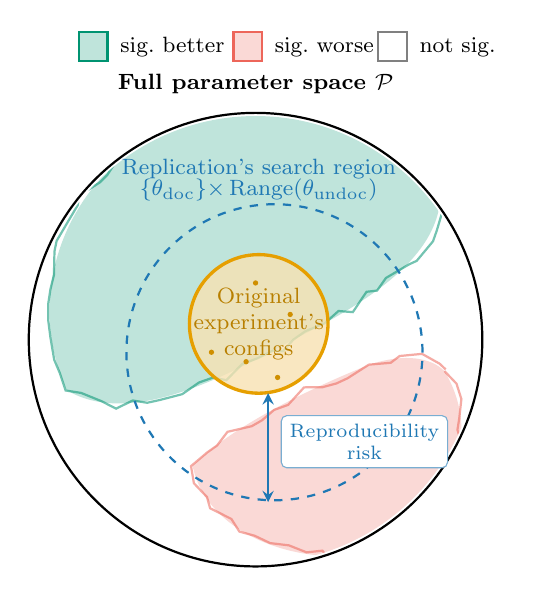
\begin{tikzpicture}[scale=0.80, every node/.style={font=\small}]

    % === Legend (above the outer circle) ===
    \begin{scope}[shift={(0,4.6)}]
      \fill[lfdTeal!25] (-2.8,-0.18) rectangle (-2.35,0.28);
      \draw[lfdTeal,thick] (-2.8,-0.18) rectangle (-2.35,0.28);
      \node[right,font=\footnotesize] at (-2.30, 0.05) {sig.\ better};
      \fill[lfdRed!25] (-0.35,-0.18) rectangle (0.10,0.28);
      \draw[lfdRed,thick] (-0.35,-0.18) rectangle (0.10,0.28);
      \node[right,font=\footnotesize] at (0.15, 0.05) {sig.\ worse};
      % \fill[gray!20] (1.95,-0.18) rectangle (2.40,0.28);
      \draw[gray,thick] (1.95,-0.18) rectangle (2.40,0.28);
      \node[right,font=\footnotesize] at (2.45, 0.05) {not sig.};
    \end{scope}

    % === Full parameter space (outer boundary) ===
    \fill[white] (0,0) circle (3.6);
    \draw[thick] (0,0) circle (3.6);
    \node[anchor=south, font=\footnotesize\bfseries] at (0,3.75)
      {Full parameter space $\mathcal{P}$};

    % === Verdict regions as organic shapes ===
    % --- "Significantly better" region (teal, upper-left; right side extended) ---
    \begin{scope}
      \clip (0,0) circle (3.55);
      \fill[lfdTeal!25]
        (-0.3,3.8) .. controls (-2.8,3.2) and (-3.8,1.0) ..
        (-3.0,-0.8) .. controls (-2.0,-1.4) and (-0.5,-0.6) ..
        (0.6,0.0) .. controls (2.2,0.8) and (3.6,1.8) ..
        (2.6,3.3) .. controls (1.6,3.9) and (0.2,3.9) .. cycle;
      \draw[lfdTeal, thick, opacity=0.55,
            decorate, decoration={random steps, segment length=6pt, amplitude=2pt}]
        (-0.3,3.8) .. controls (-2.8,3.2) and (-3.8,1.0) ..
        (-3.0,-0.8) .. controls (-2.0,-1.4) and (-0.5,-0.6) ..
        (0.6,0.0) .. controls (2.2,0.8) and (3.6,1.8) ..
        (2.6,3.3) .. controls (1.6,3.9) and (0.2,3.9) .. cycle;
    \end{scope}

    % --- "Significantly worse" region (red, bottom-right) ---
    \begin{scope}
      \clip (0,0) circle (3.55);
      \fill[lfdRed!25]
        (3.0,-0.5) .. controls (3.6,-1.5) and (3.2,-2.8) ..
        (1.8,-3.4) .. controls (0.5,-3.6) and (-0.8,-3.0) ..
        (-1.0,-2.0) .. controls (-0.4,-1.4) and (0.8,-0.8) ..
        (1.8,-0.4) .. controls (2.4,-0.2) and (2.8,-0.3) .. cycle;
      \draw[lfdRed, thick, opacity=0.55,
            decorate, decoration={random steps, segment length=6pt, amplitude=2pt}]
        (3.0,-0.5) .. controls (3.6,-1.5) and (3.2,-2.8) ..
        (1.8,-3.4) .. controls (0.5,-3.6) and (-0.8,-3.0) ..
        (-1.0,-2.0) .. controls (-0.4,-1.4) and (0.8,-0.8) ..
        (1.8,-0.4) .. controls (2.4,-0.2) and (2.8,-0.3) .. cycle;
    \end{scope}

    % === Reader's reproduction circle (slightly larger, dashed) ===
    \draw[lfdBlue, thick, dashed] (0.3,-0.2) circle (2.35);
    \node[lfdBlue, font=\footnotesize, align=center, anchor=south]
      at (0.05, 2.05)
      {Replication's search region\\[-2pt]
       $\{\theta_\text{doc}\}{\times}\,\mathrm{Range}(\theta_\text{undoc})$};

    % === Author's tested configurations (small, solid) ===
    \fill[lfdOrange!30, opacity=0.8] (0.05,.25) circle (1.1);
    \draw[lfdOrange, very thick] (0.05,.25) circle (1.1);
    \node[lfdOrange!80!black, font=\footnotesize, align=center] at (0.05,.25)
      {Original\\ experiment's\\ configs};

    % === Small dots representing individual tested configs ===
    \foreach \x/\y in {
      0/.9, 0.55/.4, 0.35/-.6, -0.15/-.35, -0.7/-.2} {
      \fill[lfdOrange!90!black] (\x,\y) circle (1.2pt);
    }

    % === Annotation arrow: reproducibility risk ===
    \draw[<->, >=stealth, thick, lfdBlue]
      (0.2, -0.85) -- (0.2, -2.58);
    \node[lfdBlue, font=\scriptsize, align=center,
          fill=white, draw=lfdBlue!60, thin, rounded corners=2pt, inner sep=3pt,
          anchor=west]
      at (0.4, -1.62) {Reproducibility\\ risk};
\end{tikzpicture}
\end{document}
